\section{Motivation}

\begin{frame}
    \frametitle{What is hardware isolation?}

    \begin{center}
        \textbf{Limiting access of hardware (and software) to needed resources}
    \end{center}
\end{frame}

\begin{frame}
    \frametitle{Why hardware isolation?}

    Traditional hardware model:

    \begin{itemize}
        \item Internal and external hardware is considered trustworthy
        \item Hardware has unrestricted access to other hardware, e.g., network
            cards to main memory
        \item Software with direct access to hardware (e.g., drivers) may
            (ab-)use the capabilities of the controlled hardware
    \end{itemize}

    \vspace{1em}

    Unrestricted hardware access to memory is a problem:

    \begin{itemize}
%        \item Virtual machines may access memory of other virtual machines
        \item Malicious devices or drivers may leak secret data from memory
        \item Faulty devices or drivers may corrupt OS data structures and crash the system
    \end{itemize}
\end{frame}

% \begin{frame}
%     \frametitle{Why hardware isolation?}
% 
%     Hardware can be isolated through ...
% 
%     \begin{itemize}
%         \item Software, e.g., a VM hypervisor, by restricting access to the hardware
%         \item Hardware, e.g., by special components that restrict access of
%             other components
%     \end{itemize}
% 
%     \vspace{0.75cm}
% 
%     Hardware isolation thus reduces the attack surface for ...
% 
%     \begin{itemize}
%         \item Virtual machines, containers, network function virtualization
%         \item Untrusted hardware and untrusted drivers
%     \end{itemize}
% \end{frame}

\begin{frame}
    \frametitle{How is hardware interconnected on modern systems?}

    \only<1>{
        \begin{figure}
            \centering
            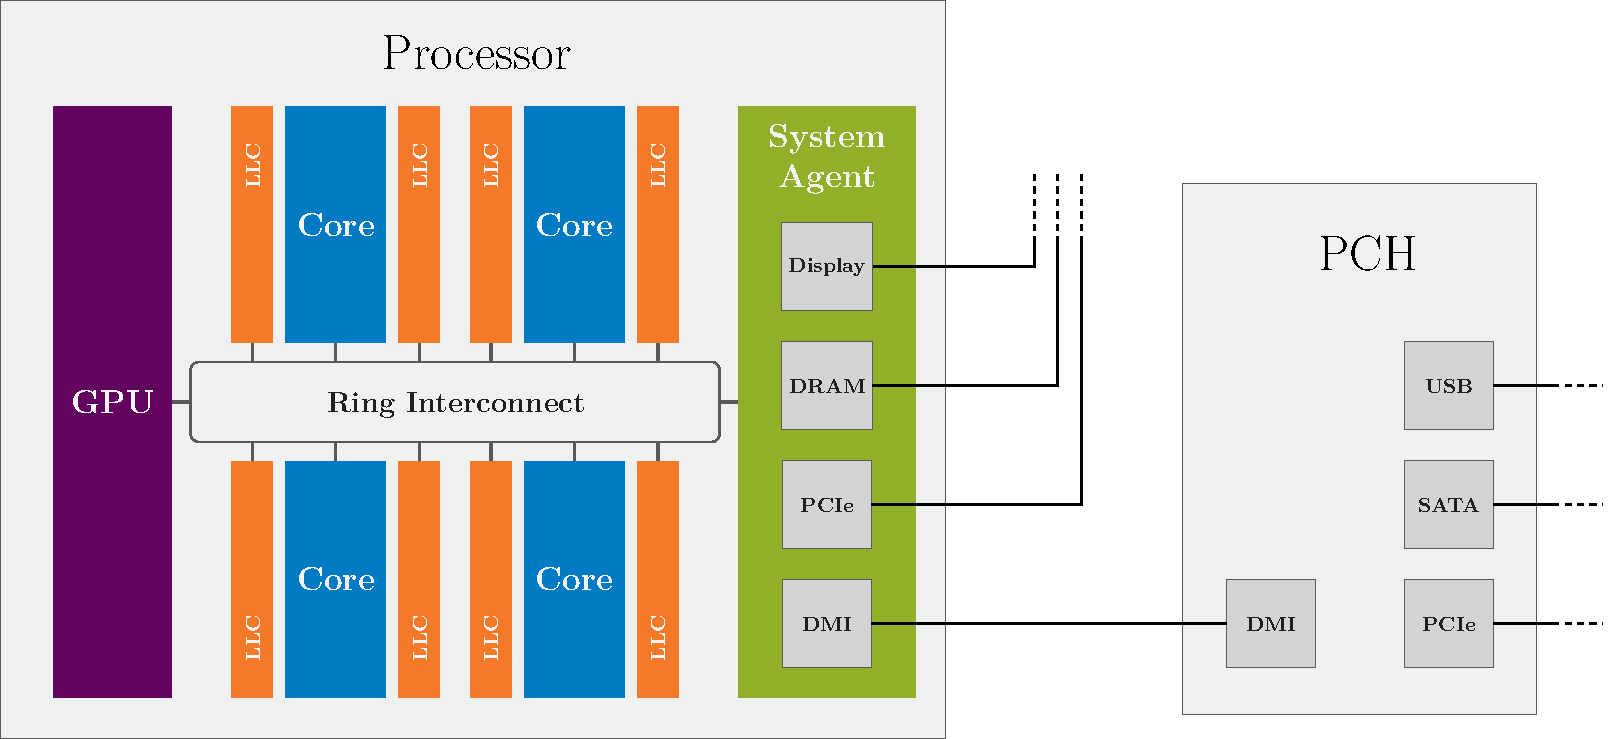
\includegraphics[width=0.9\textwidth,clip]{figures/cpu-and-pch.pdf}
        \end{figure}
    }

    \only<2>{
        \begin{figure}
            \centering
            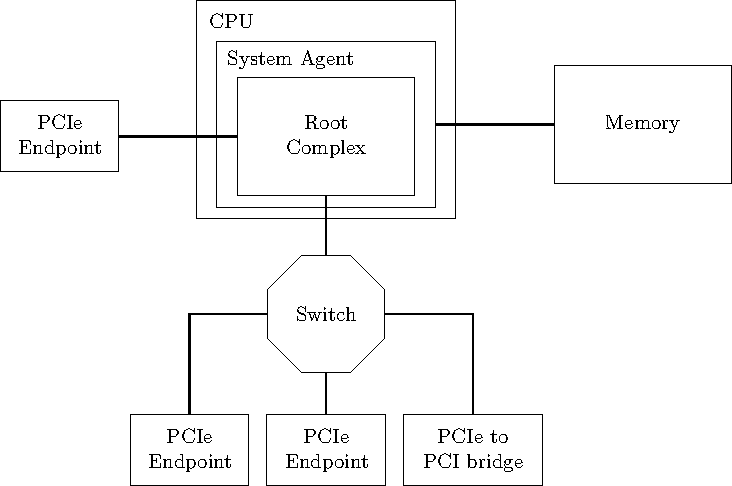
\includegraphics[width=0.7\textwidth,clip]{figures/pcie-tree.pdf}
        \end{figure}
    }
\end{frame}

\begin{frame}
    \frametitle{How do peripherals access main memory?}

    \begin{itemize}
        \item Devices use direct memory access (DMA) to access main memory without
            CPU involvement
        \item In case of PCIe, devices issue memory read/write requests to the
            root complex
        \item DMA requests address memory through physical addresses
    \end{itemize}
\end{frame}

% \begin{frame}
%     \frametitle{How to isolate hardware?}
% 
%     Unrestricted hardware access to main memory can be mitigated:
% 
%     \begin{itemize}
%         \item Through software, e.g., hypervisor (VMM) monitoring all IO operations
%         \item Through hardware, e.g., MMUs for IO devices (IOMMUs)
%     \end{itemize}
% 
%      \vspace{1em}
% 
%      We will focus on isolation through hardware since isolation through
%      software is known to be slow.
%  
% %     Questions:
% % 
% %     \begin{itemize}
% %         \item Hardware isolation by software is known to be slow, how does
% %             isolation by hardware perform?
% %         \item Is isolation by hardware safe and secure?
% %     \end{itemize}
% \end{frame}

\begin{frame}
    \frametitle{Hardware can be isolated through IOMMUs}

    Input-Output Memory Management Units (IOMMUs):

    \begin{itemize}
        \item Translate IO virtual addresses (IOVA) to physical addresses (PA)
        \item Restrict access of IO devices to assigned address space
    \end{itemize}

    \vspace{1em}
    Advantages:

    \begin{itemize}
        \item Limit effects of faulty or malicious devices/software
        \item Contiguous virtual address space does not have to be contiguous in
            physical memory
        \item Enable 32-bit devices to address memory above 4 GiB
        \item Allow for safe and secure direct passthrough of hardware to virtual machines
    \end{itemize}
\end{frame}

\section{IOMMUs}

\begin{frame}
    \frametitle{Virtualization}

    \only<1>{
        \begin{figure}
            \centering
            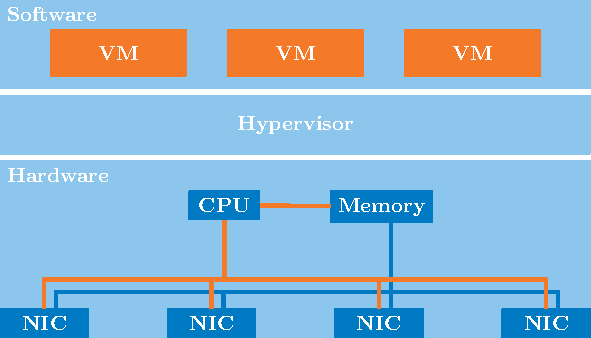
\includegraphics[width=0.8\textwidth,clip]{figures/hypervisor-vms.pdf}
        \end{figure}
    }

    \only<2>{
        \begin{figure}
            \centering
            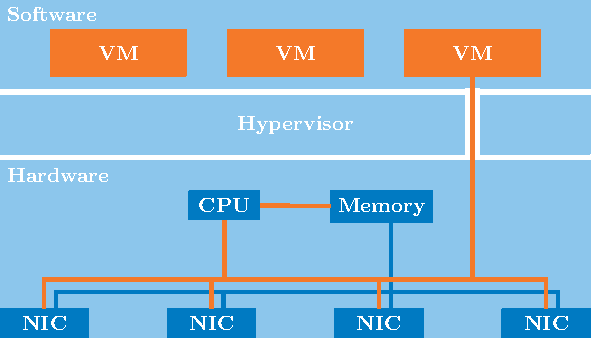
\includegraphics[width=0.8\textwidth,clip]{figures/hypervisor-vms-pt.pdf}
        \end{figure}
    }

    \only<3>{
        \begin{figure}
            \centering
            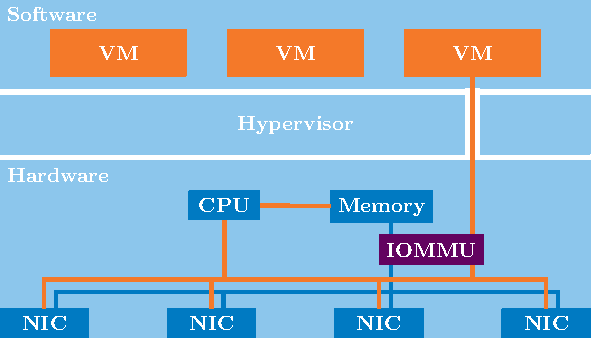
\includegraphics[width=0.8\textwidth,clip]{figures/hypervisor-vms-pt-iommu.pdf}
        \end{figure}
    }
\end{frame}

\begin{frame}
    \frametitle{Location in the PCIe tree}

    \begin{figure}
        \centering
        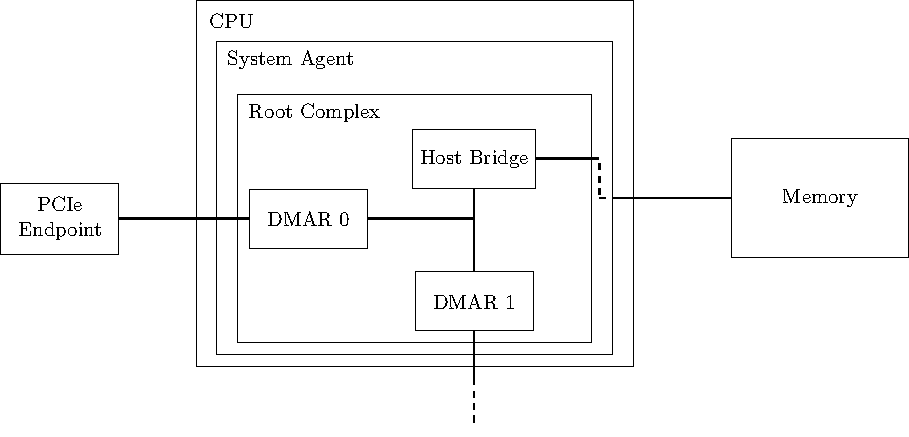
\includegraphics[width=0.9\textwidth,clip]{figures/pcie-dmar.pdf}
        \caption{IOMMUs (DMARs) in the PCIe tree.}
    \end{figure}
\end{frame}

\begin{frame}
    \frametitle{Real world use cases}

    \begin{itemize}
        \item Amazon's Elastic Compute Cloud provides 10G networking through
            SR-IOV + IOMMUs
        \item MacBooks use IOMMUs to protect themselves against external
            Thunderbolt devices
        \item iPhones have an IOMMU included to isolate the WiFi stack
    \end{itemize}

    \vspace{3em}

    \begin{center}
        \begin{minipage}{0.35\textwidth}
            \begin{figure}
                
\includegraphics[width=0.4\textwidth]{pics/aws.png}
            \end{figure}
        \end{minipage}%
        \begin{minipage}{0.35\textwidth}
            \begin{figure}
                
\includegraphics[width=0.22\textwidth]{pics/thunderbolt.png}
            \end{figure}
        \end{minipage}
    \end{center}
\end{frame}


\section{Research Questions}

\begin{frame}
    Reasons to have a closer look at IOMMUs:

    \begin{itemize}
        \item Documentation about IOMMU implementations is sparse
        \item Some publications report huge performance impacts and
            vulnerabilities
        \item Differences of IOMMUs from different vendors (Intel, AMD, ARM, ...)
            mostly unknown
        \item Increasing prevalence of IOMMUs in servers, home computers and
            mobile devices
    \end{itemize}

    \vspace{1em}

    Key question of our work:
    
    \begin{itemize}
        \item What is the trade-off between performance and safety/security in
            high-speed network environments?
    \end{itemize}
\end{frame}


\section{Methodology}

\begin{frame}
    \frametitle{How to determine performance effects of IOMMUs?}

    \begin{itemize}
        \item Desirable properties in high-speed networks are high packet
            throughput rates and low latency
        \item To determine negative effects on these properties we need some
            application that provides high throughput rates and low latency
        \item Why not use a user space network driver?
    \end{itemize}
\end{frame}

\begin{frame}
    \frametitle{Test setup}

    \begin{minipage}{0.5\textwidth}
        Benchmarking IOMMUs with ixy.rs:

        \begin{itemize}
            \item state-of-the-art user space network driver
            \item can forward >\SI{26}{Mpps} on a single \SI{3.3}{\giga\hertz}
                CPU core
            \item less than 2,000 lines of code
            \item written in Rust
        \end{itemize}

        \vspace{2em}

        Missing in ixy.rs:

        \begin{itemize}
            \item Support for SR-IOV
            \item Support for legacy IOMMUs with small IOVA widths
        \end{itemize}
    \end{minipage}%
    \begin{minipage}[c]{0.5\textwidth}
        \begin{figure}
            \centering
            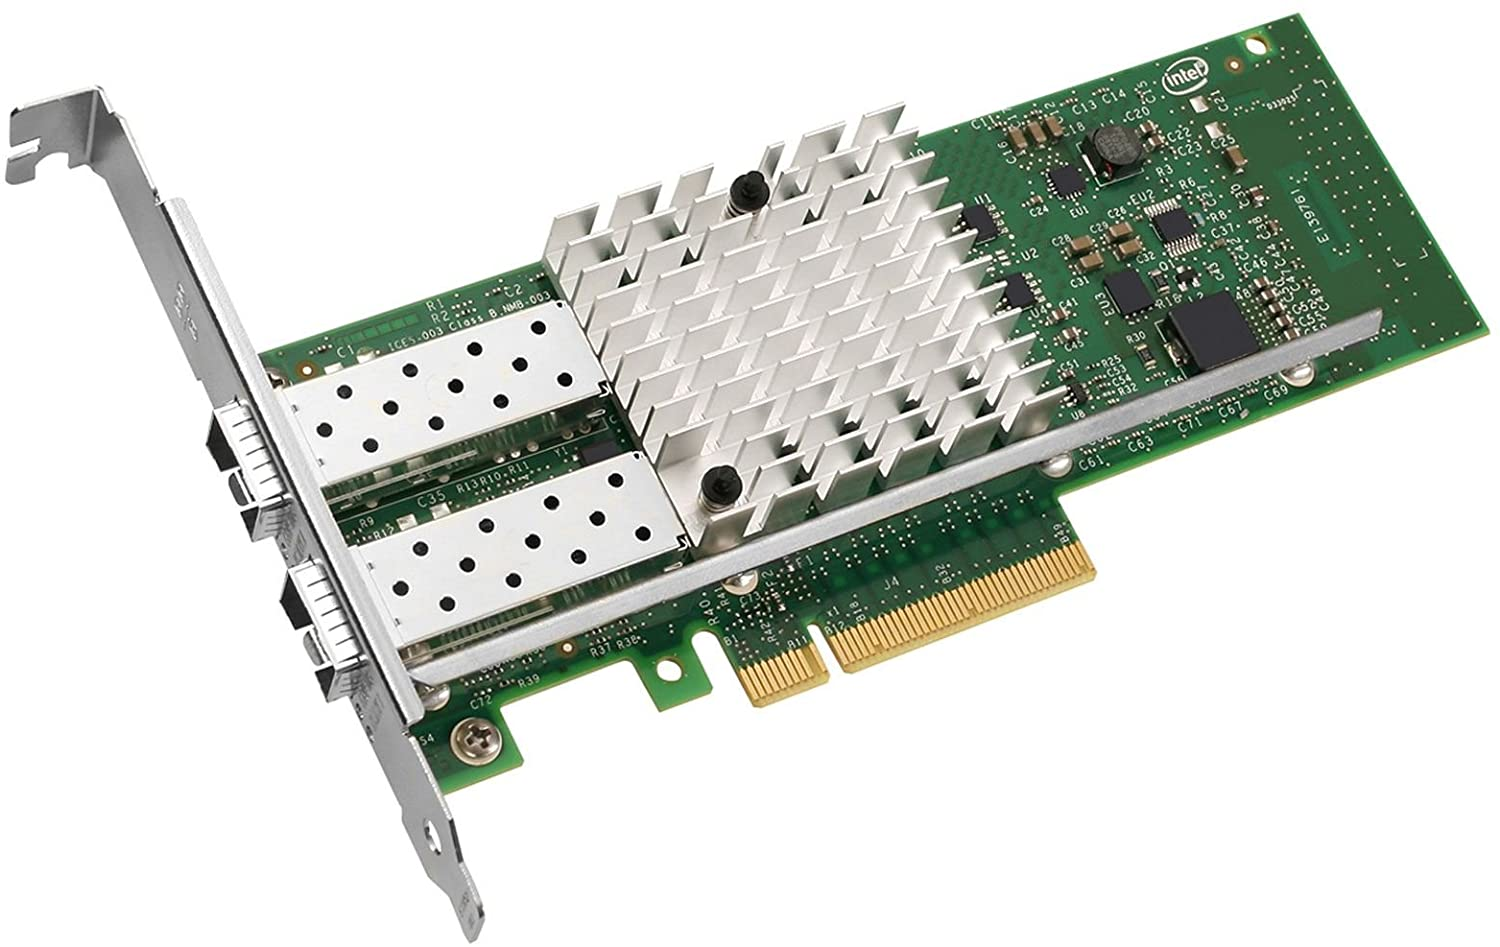
\includegraphics[width=0.8\textwidth,clip,trim=0cm 0cm 0cm
            0cm]{pics/intel_x520_da2.jpg}
            \caption{Intel X520-DA2 [Picture: amazon.com]}
        \end{figure}
    \end{minipage}
\end{frame}

\begin{frame}
    \frametitle{Test setup}

    \centering\includestandalone[scale=0.65]{figures/testsetup}
\end{frame}

\begin{frame}
    \frametitle{Devices under test}

    \only<1>{
        \begin{table}
            \centering
            \begin{tabular}{lllrll}
                \textbf{CPU} & \textbf{Year} & \textbf{Arch.} & \textbf{Memory} & \textbf{NIC} & \textbf{NUMA} \\
                \toprule

                \multirow{2}{*}{Intel Xeon E3-1230v2} & \multirow{2}{*}{2012} &
                \multirow{2}{*}{Ivy Bridge} & \multirow{2}{*}{\SI{16}{\giga\byte}} & Intel X520-DA1 &
                \multirow{2}{*}{no} \\
                & & & & Intel X520-DA2 & \\ \hline

                \multirow{2}{*}{Intel Xeon E5-2620v3} & \multirow{2}{*}{2014} &
                \multirow{2}{*}{Haswell} & \multirow{2}{*}{\SI{32}{\giga\byte}} & Intel X520-DA2 &
                \multirow{2}{*}{no} \\
                & & & & Intel X540-T2 & \\ \hline

                \multirow{2}{*}{AMD EPYC 7551P} & \multirow{2}{*}{2017} &
                \multirow{2}{*}{Naples} & \multirow{2}{*}{\SI{128}{\giga\byte}} & Intel X550T &
                \multirow{2}{*}{yes} \\
                & & & & Intel X550T & \\

                \bottomrule
            \end{tabular}
        \end{table}
    }

    \only<2>{
        \begin{table}
            \centering
            \begin{tabular}{llrrrr}
                \multirow{2}{*}{\textbf{CPU}} & \multirow{2}{*}{\textbf{Clock}} &
                \multirow{2}{*}{\textbf{Cores}} & \multirow{2}{*}{\textbf{L3-Cache}} &
                \multicolumn{2}{r}{\textbf{PassMark}} \\
                & & & & \textbf{ST} & \textbf{All} \\
                \toprule

                Intel Xeon E3-1230v2 & \SI{3.3}{\giga\Hz} &  4 &  \SI{8}{\mega\byte} & 1,996 &  6,192 \\
                Intel Xeon E5-2620v3 & \SI{2.4}{\giga\Hz} &  6 & \SI{15}{\mega\byte} & 1,700 &  7,979 \\
                AMD EPYC 7551P       & \SI{2.0}{\giga\Hz} & 32 & \SI{64}{\mega\byte} & 1,611 & 25,933 \\

                \bottomrule
            \end{tabular}

            \label{tab:cpus}
        \end{table}
    }
\end{frame}

\section{Performance Analysis}

\begin{frame}
    \frametitle{Baseline performance of devices under test}

    \only<1>{
        Idea:

        \begin{itemize}
            \item Determine performance of devices under test without modifications
            \item Detect unusual behaviour, e.g., exceptionally good/bad performance
        \end{itemize}
    }

    \only<2>{
        \begin{figure}
            \centering
            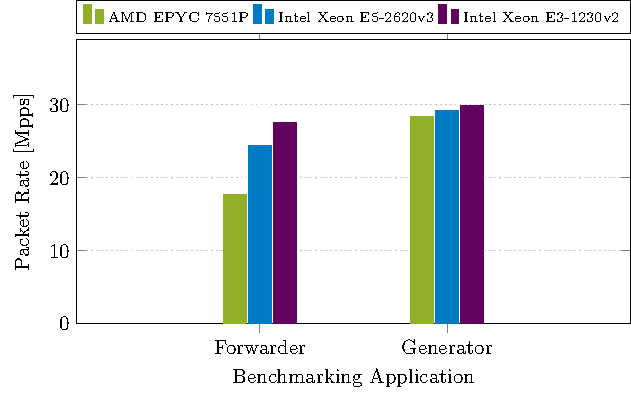
\includegraphics[width=0.7\textwidth,clip]{figures/baseline-throughput.pdf}
            \caption{Baseline throughput of ixy.rs on devices under test without
            IOMMU.}
        \end{figure}
    }

    % \only<3>{
    %     \begin{figure}
    %         \centering
    %         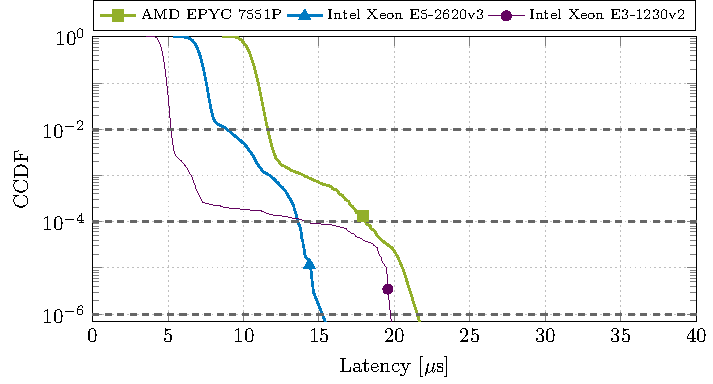
\includegraphics[width=0.8\textwidth,clip]{figures/baseline-latency.pdf}
    %         \caption{Baseline latency of forwarder on devices under test without
    %             IOMMU.\\Measured with a load of \SI{10}{Mpps}.}
    %     \end{figure}
    % }

    \only<3>{
        Results:

        \begin{itemize}
            \item Throughput rates reflect clock speeds of the CPUs
            \item Forwarder on AMD EPYC CPU is significantly slower than expected
        \end{itemize}

        \vspace{1em}

        Reasons for the relatively poor performance of AMD EPYC:
        
        \begin{itemize}
            \item 1/6 less instructions per cycle than Intel Xeon E5
            \item 12-39x more branch mispredictions
            \item probably 1-2 additional cycles per branch misprediction (at least
                on Zen 2)
        \end{itemize}
    }
\end{frame}

\begin{frame}
    \frametitle{Throughput with different page sizes}

    \only<1>{
    Idea:

    \begin{itemize}
        \item IOMMUs cache translations in I/O translation lookaside buffers (IOTLBs)
        \item Can we determine the number of pages cached in the IOTLB?
        \item With too many pages, throughput may drop due to the IOTLB getting thrashed
    \end{itemize}
    }

    \only<2>{
        \begin{figure}
            \centering
            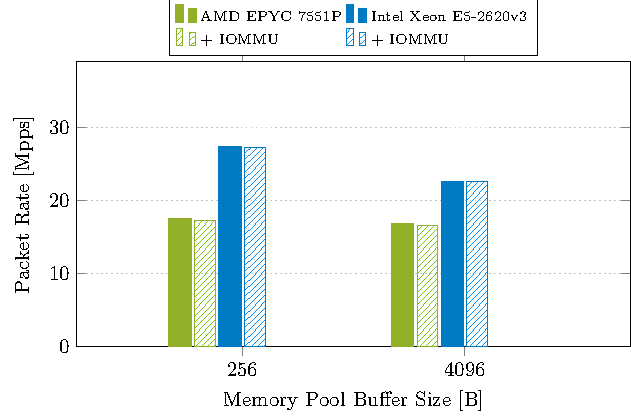
\includegraphics[width=0.7\textwidth,clip]{figures/page-size-1g-throughput.pdf}
            \caption{Throughput of forwarder with \SI{1}{\gibi\byte} pages. Two
                pools with 512 buffers each used.}
        \end{figure}
    }

    \only<3>{
        \begin{figure}
            \centering
            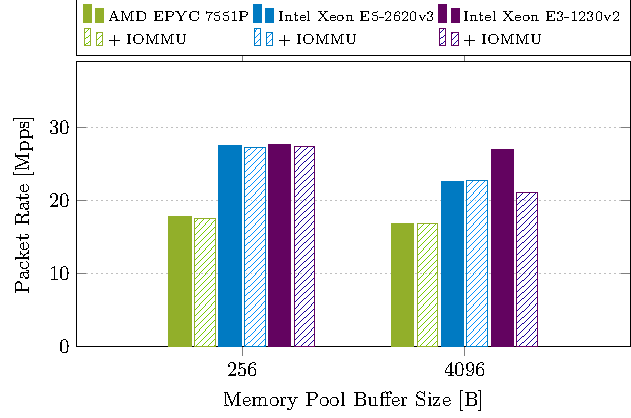
\includegraphics[width=0.7\textwidth,clip]{figures/page-size-2m-throughput.pdf}
            \caption{Throughput of forwarder with \SI{2}{\mebi\byte} pages. Two
                pools with 512 buffers each used.}
        \end{figure}
    }

    \only<4>{
        \begin{figure}
            \centering
            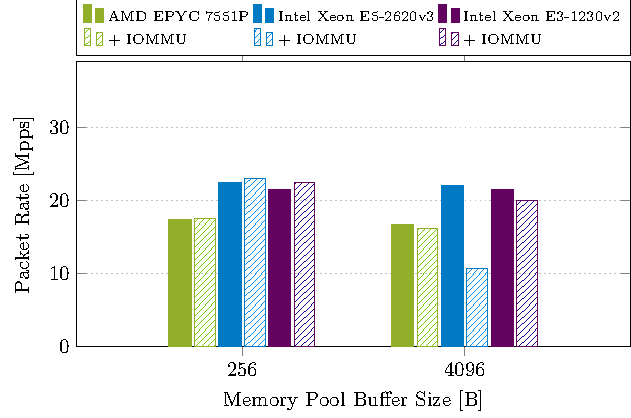
\includegraphics[width=0.7\textwidth,clip]{figures/page-size-4k-throughput.pdf}
            \caption{Throughput of forwarder with \SI{4}{\kibi\byte} pages. Two
                pools with 512 buffers each used.}
        \end{figure}
    }

    \only<5>{
        \begin{figure}
            \centering
            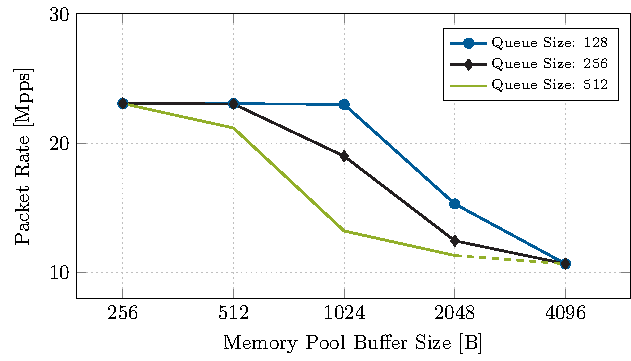
\includegraphics[width=0.7\textwidth,clip]{figures/page-size-4k-omanyte-throughput.pdf}
            \caption{Throughput of forwarder on Intel Xeon E5 with
                \SI{4}{\kibi\byte} pages and IOMMU enabled. Pool size = 2 x queue size.}
        \end{figure}
    }

    \only<6>{
        \begin{figure}%[!b]
            \centering
            \subfloat[No IOMMU]{%
                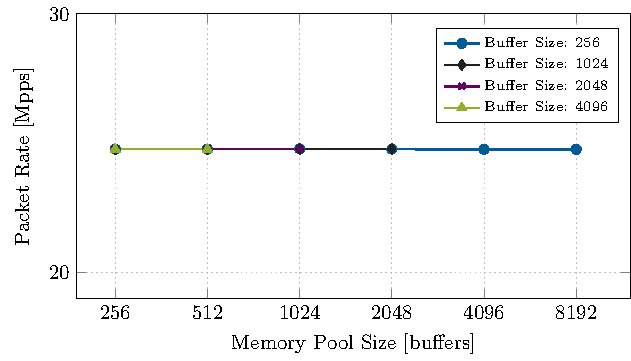
\includegraphics[width=0.46\textwidth,clip]{figures/page-size-4k-omanyte-generator-two-throughput.pdf}
            }
            \subfloat[IOMMU]{%
                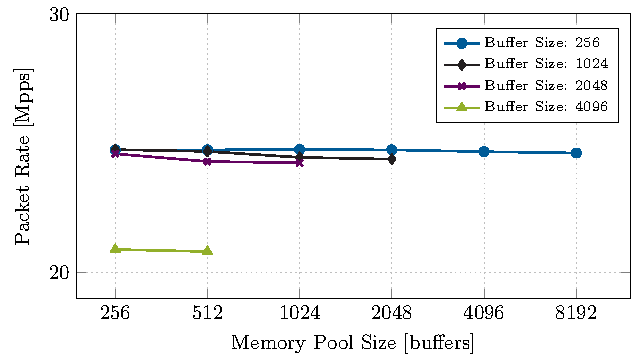
\includegraphics[width=0.46\textwidth,clip]{figures/page-size-4k-omanyte-generator-iommu-two-throughput.pdf}
            }

            \caption{Packet rate of generators on Intel Xeon E5 with
            \SI{4}{\kibi\byte} pages.}
        \end{figure}
    }

    \only<7>{
        Results:

        \begin{itemize}
            \item Page sizes have no major effect on throughput on AMD EPYC and Intel Xeon E3
            \item IOTLB seems to get thrashed on the Intel Xeon E5-2620v3 when using
                more than 64 pages
            \item Neugebauer et al. determined an IOTLB size of 64 entries for their
                Intel Xeon E5-2630v4
            \item However, our packet generator does not show any correlation
                between number of used pages and packet rate
        \end{itemize}
    }
\end{frame}

\begin{frame}
    \frametitle{Throughput with different IOVA address widths}

    \only<1>{
        Idea:

        \begin{itemize}
            \item Depending on IOVA address widths, IOMMUs use different translation
                structures
            \item Does the number of page tables to be walked affect performance?
        \end{itemize}
    }

    \only<2>{
        \begin{figure}
            \centering
            \subfloat[Using 2 ports of the same NIC]{%
                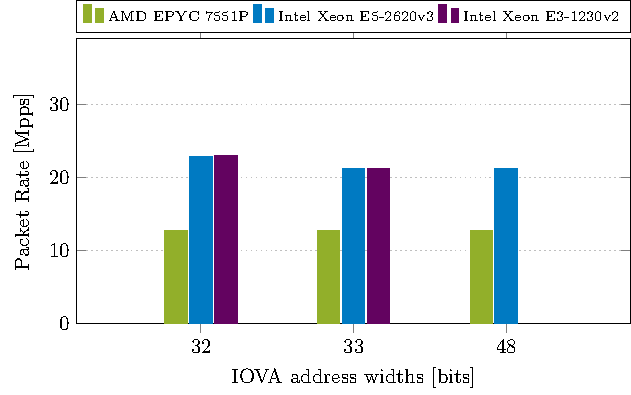
\includegraphics[width=0.46\textwidth,clip]{figures/iova-address-widths-single-device-throughput.pdf}
            }
            \subfloat[Using 2 ports of different NICs]{%
                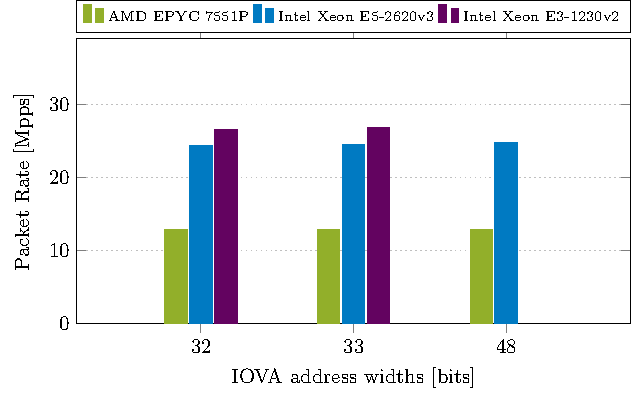
\includegraphics[width=0.46\textwidth,clip]{figures/iova-address-widths-two-devices-throughput.pdf}
            }

            \caption{Throughput of forwarder with 32, 33 and \SI{48}{\bit} wide IOVAs.}
        \end{figure}
    }

    \only<3>{
        Results:

        \begin{itemize}
            \item IOVA address widths do not affect performance when using two
                different NICs
            \item Larger IOVA addresses negatively affect performance when
                using two ports of the same NIC
            \item We suspect that the PCIe bus limits throughput: PCIe packets with
                32-bit addresses use \SI{4}{\byte} smaller headers
        \end{itemize}
    }
\end{frame}

\begin{frame}
    \frametitle{Throughput with SR-IOV}

    \only<1>{
        Servers use Single-Root Input-Output Virtualization (SR-IOV) to pass a
        single network card to multiple virtual machines by splitting the device
        into multiple so-called virtual functions (VFs).

        \vspace{2em}

        Idea:

        \begin{itemize}
            \item Do IOMMUs affect throughput when using SR-IOV?
        \end{itemize}
    }

    \only<2>{
        \begin{figure}
            \centering
            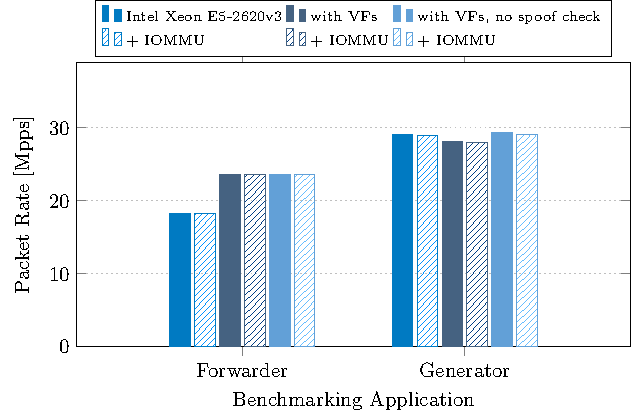
\includegraphics[width=0.7\textwidth]{figures/sriov-omanyte-throughput.pdf}
            \caption{Throughput of SRIOV-modified forwarder on Intel Xeon E5.}
        \end{figure}
    }

    \only<3>{
        \begin{figure}
            \centering
            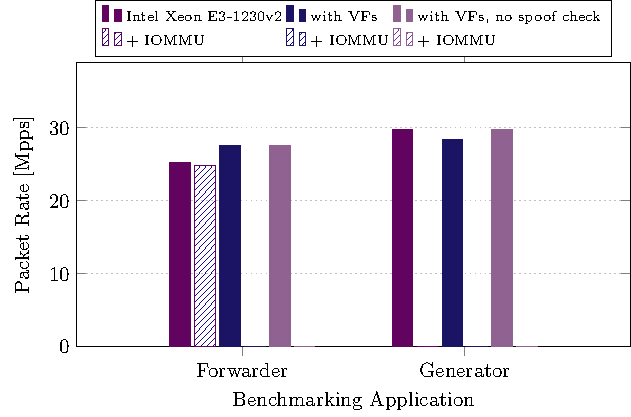
\includegraphics[width=0.7\textwidth]{figures/sriov-narva-throughput.pdf}
            \caption{Throughput of SRIOV-modified forwarder on Intel Xeon E3.}
        \end{figure}
    }

    \only<4>{
        Results:

        \begin{itemize}
            \item IOMMUs do not affect throughput using SR-IOV
        \end{itemize}
    }
\end{frame}

\section{Safety and Security}

\begin{frame}
    \frametitle{Known vulnerabilities}

    \only<1>{
        PCIe is inherently unsafe:

        \begin{itemize}
            \item PCIe devices can impersonate other devices by using their PCIe IDs
            \item PCIe devices may announce Address Translation Services (ATS)
                support
        \end{itemize}

        \vspace{1em}

        Address Translation Services (ATS):

        \begin{itemize}
            \item Devices cache IOMMU address translations to reduce pressure on IOTLB
            \item Addresses in PCIe requests are marked as already translated
            \item PCIe requests with translated addresses are not checked by the
                IOMMU, i.e., devices have unrestricted access to main memory
            \item Linux disabled ATS for external devices (e.g., Thunderbolt) in
                2018
        \end{itemize}
    }

    \only<2>{
        Architectural deficiencies:

        \begin{itemize}
            \item OSes detect hardware using ACPI tables which could be overriden at
                boot time on some systems such that IOMMUs are hidden from the OS
            \item IOMMU translation tables could be overridden on some systems
                during IOMMU initialization, disabling translation for all devices
        \end{itemize}

        \vspace{1em}

        Flaws in IOMMU usage by OSes:

        \begin{itemize}
            \item Until October 2020, Windows did not use IOMMUs at all
            \item Linux and macOS put kernel data structures into IOMMU-protected
                memory such that root shells could be obtained on both OSes
        \end{itemize}
    }
\end{frame}

\begin{frame}
    \frametitle{Are there more vulnerabilities?}

    Caches allow for timing-attacks:

    \begin{itemize}
        \item IOMMUs cache address translations in IOTLBs
        \item Can we detect whether a translation was cached in the IOTLB or a
            page table walk had to be performed?
        \item If so, can we prime the IOTLB such that we can detect whether
            other devices / virtual functions have performed a PCIe memory
            request, i.e., have received/transmitted packets?
    \end{itemize}
\end{frame}

\begin{frame}
    \frametitle{Measuring DMA access times}

    \only<1>{
        Idea:

        \begin{itemize}
            \item Continuously transmit batches of packets such that IOTLB is fully
                used
            \item Measure CPU cycles it takes to transmit the packet batches
            \item If another NIC receives or transmits a packet, at least one IOTLB
                entry is replaced by the IOMMU
            \item Transmitting the next batch of packets should take more CPU cycles
                due to IOTLB misses
        \end{itemize}
    }

    \only<2>{
        \begin{figure}
            \centering
            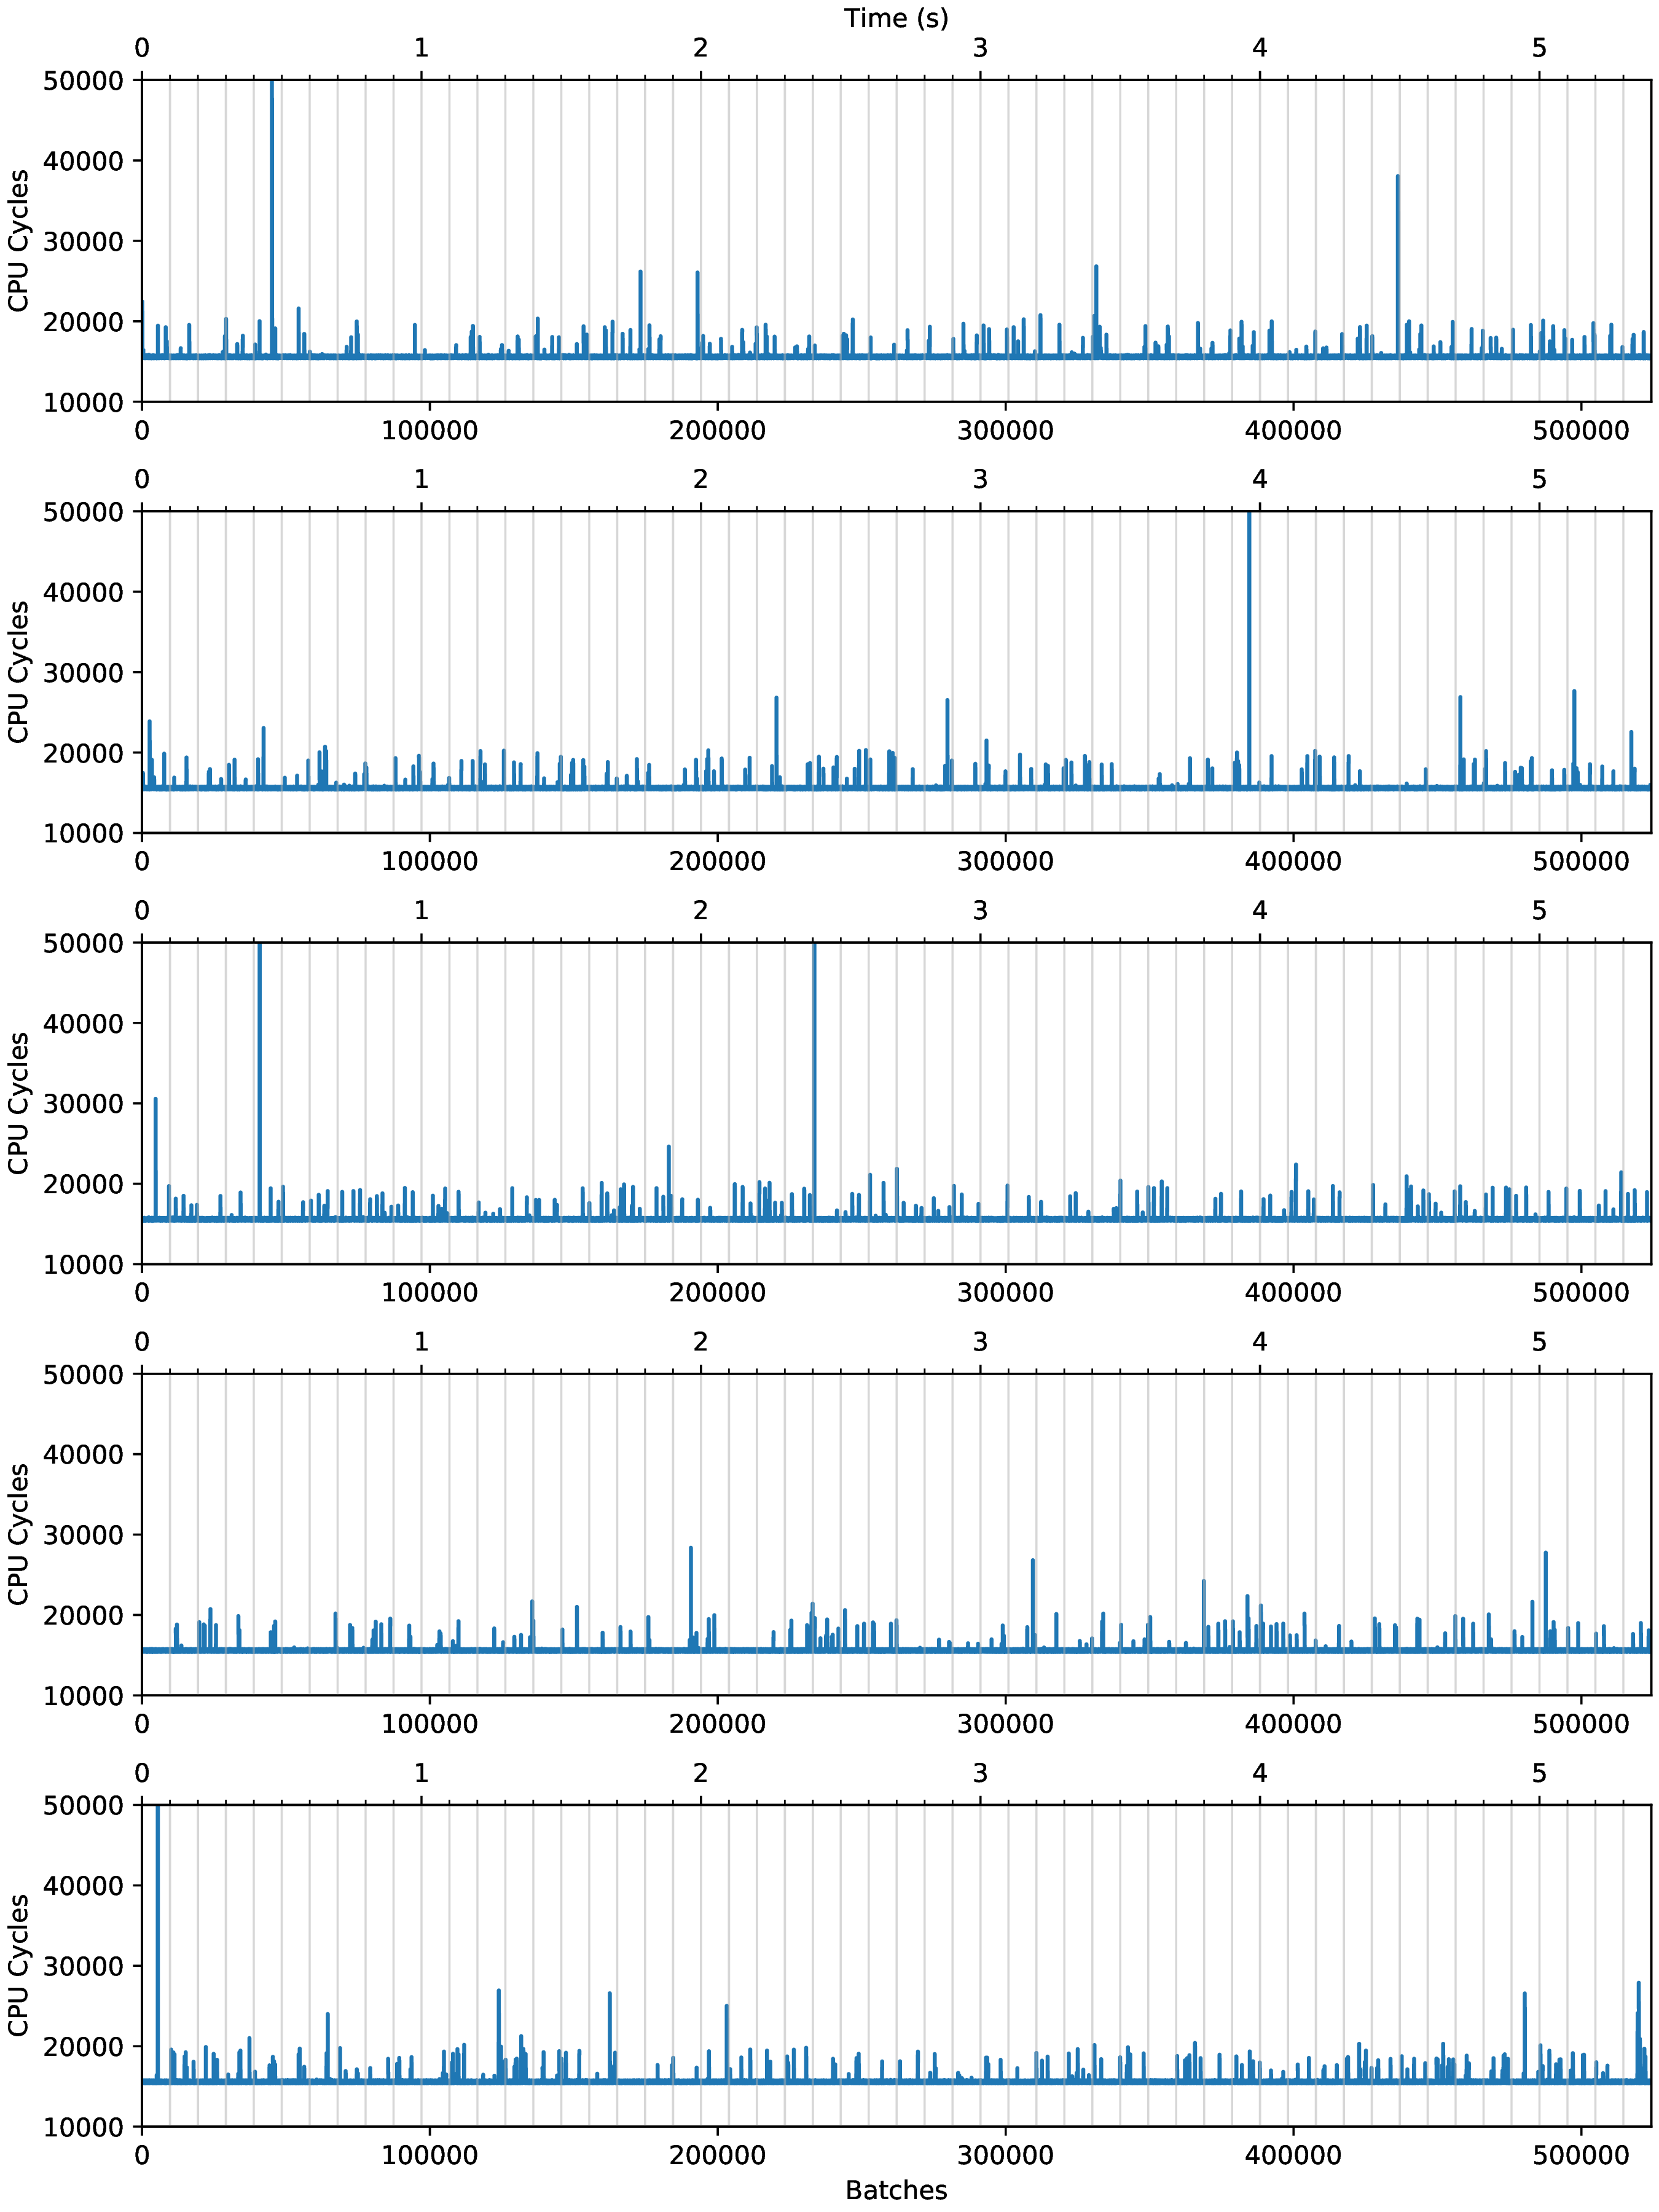
\includegraphics[width=0.7\textwidth,trim={0 52cm 0 0},clip]{figures/iotlb-baseline-no-iommu.png}
            \caption{CPU cycles per batch of transmitted packets without IOMMU.}
        \end{figure}
    }

    \only<3>{
        \begin{figure}
            \centering
            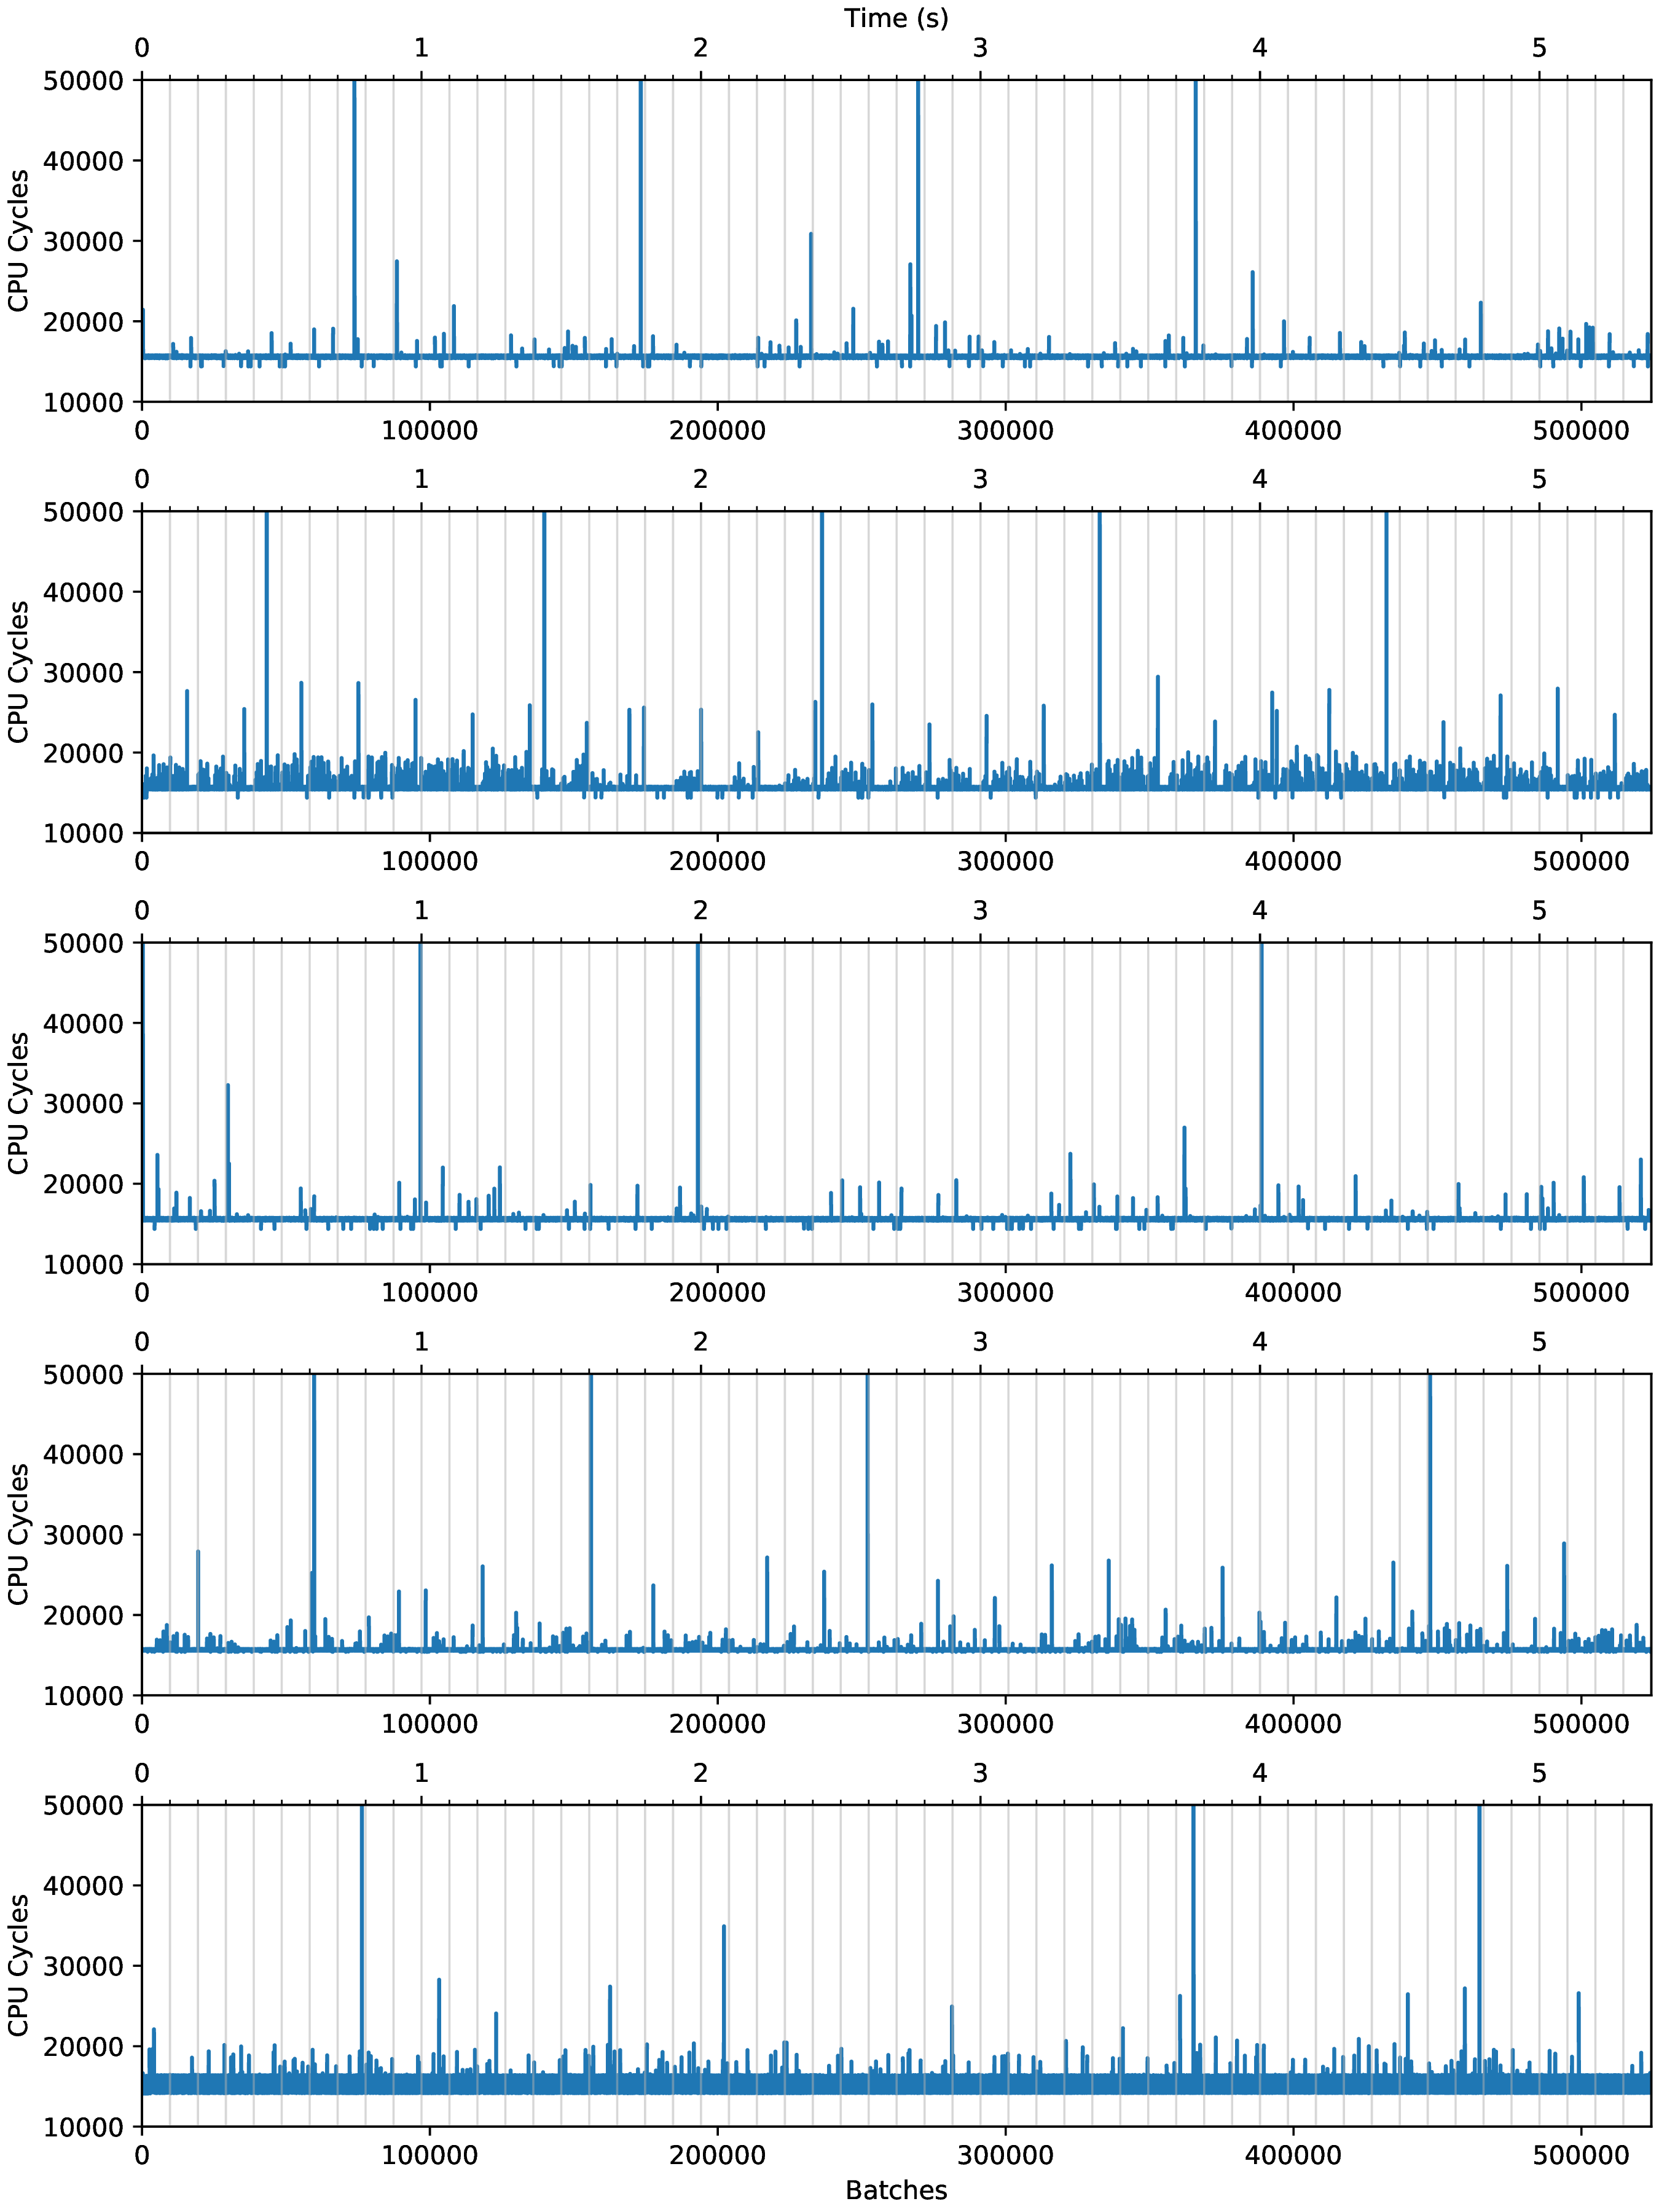
\includegraphics[width=0.7\textwidth,trim={0 52cm 0 0},clip]{figures/iotlb-baseline-iommu-pt.png}
            \caption{CPU cycles per batch of transmitted packets with IOMMU.}
        \end{figure}
    }

    \only<4>{
        \begin{figure}
            \centering
            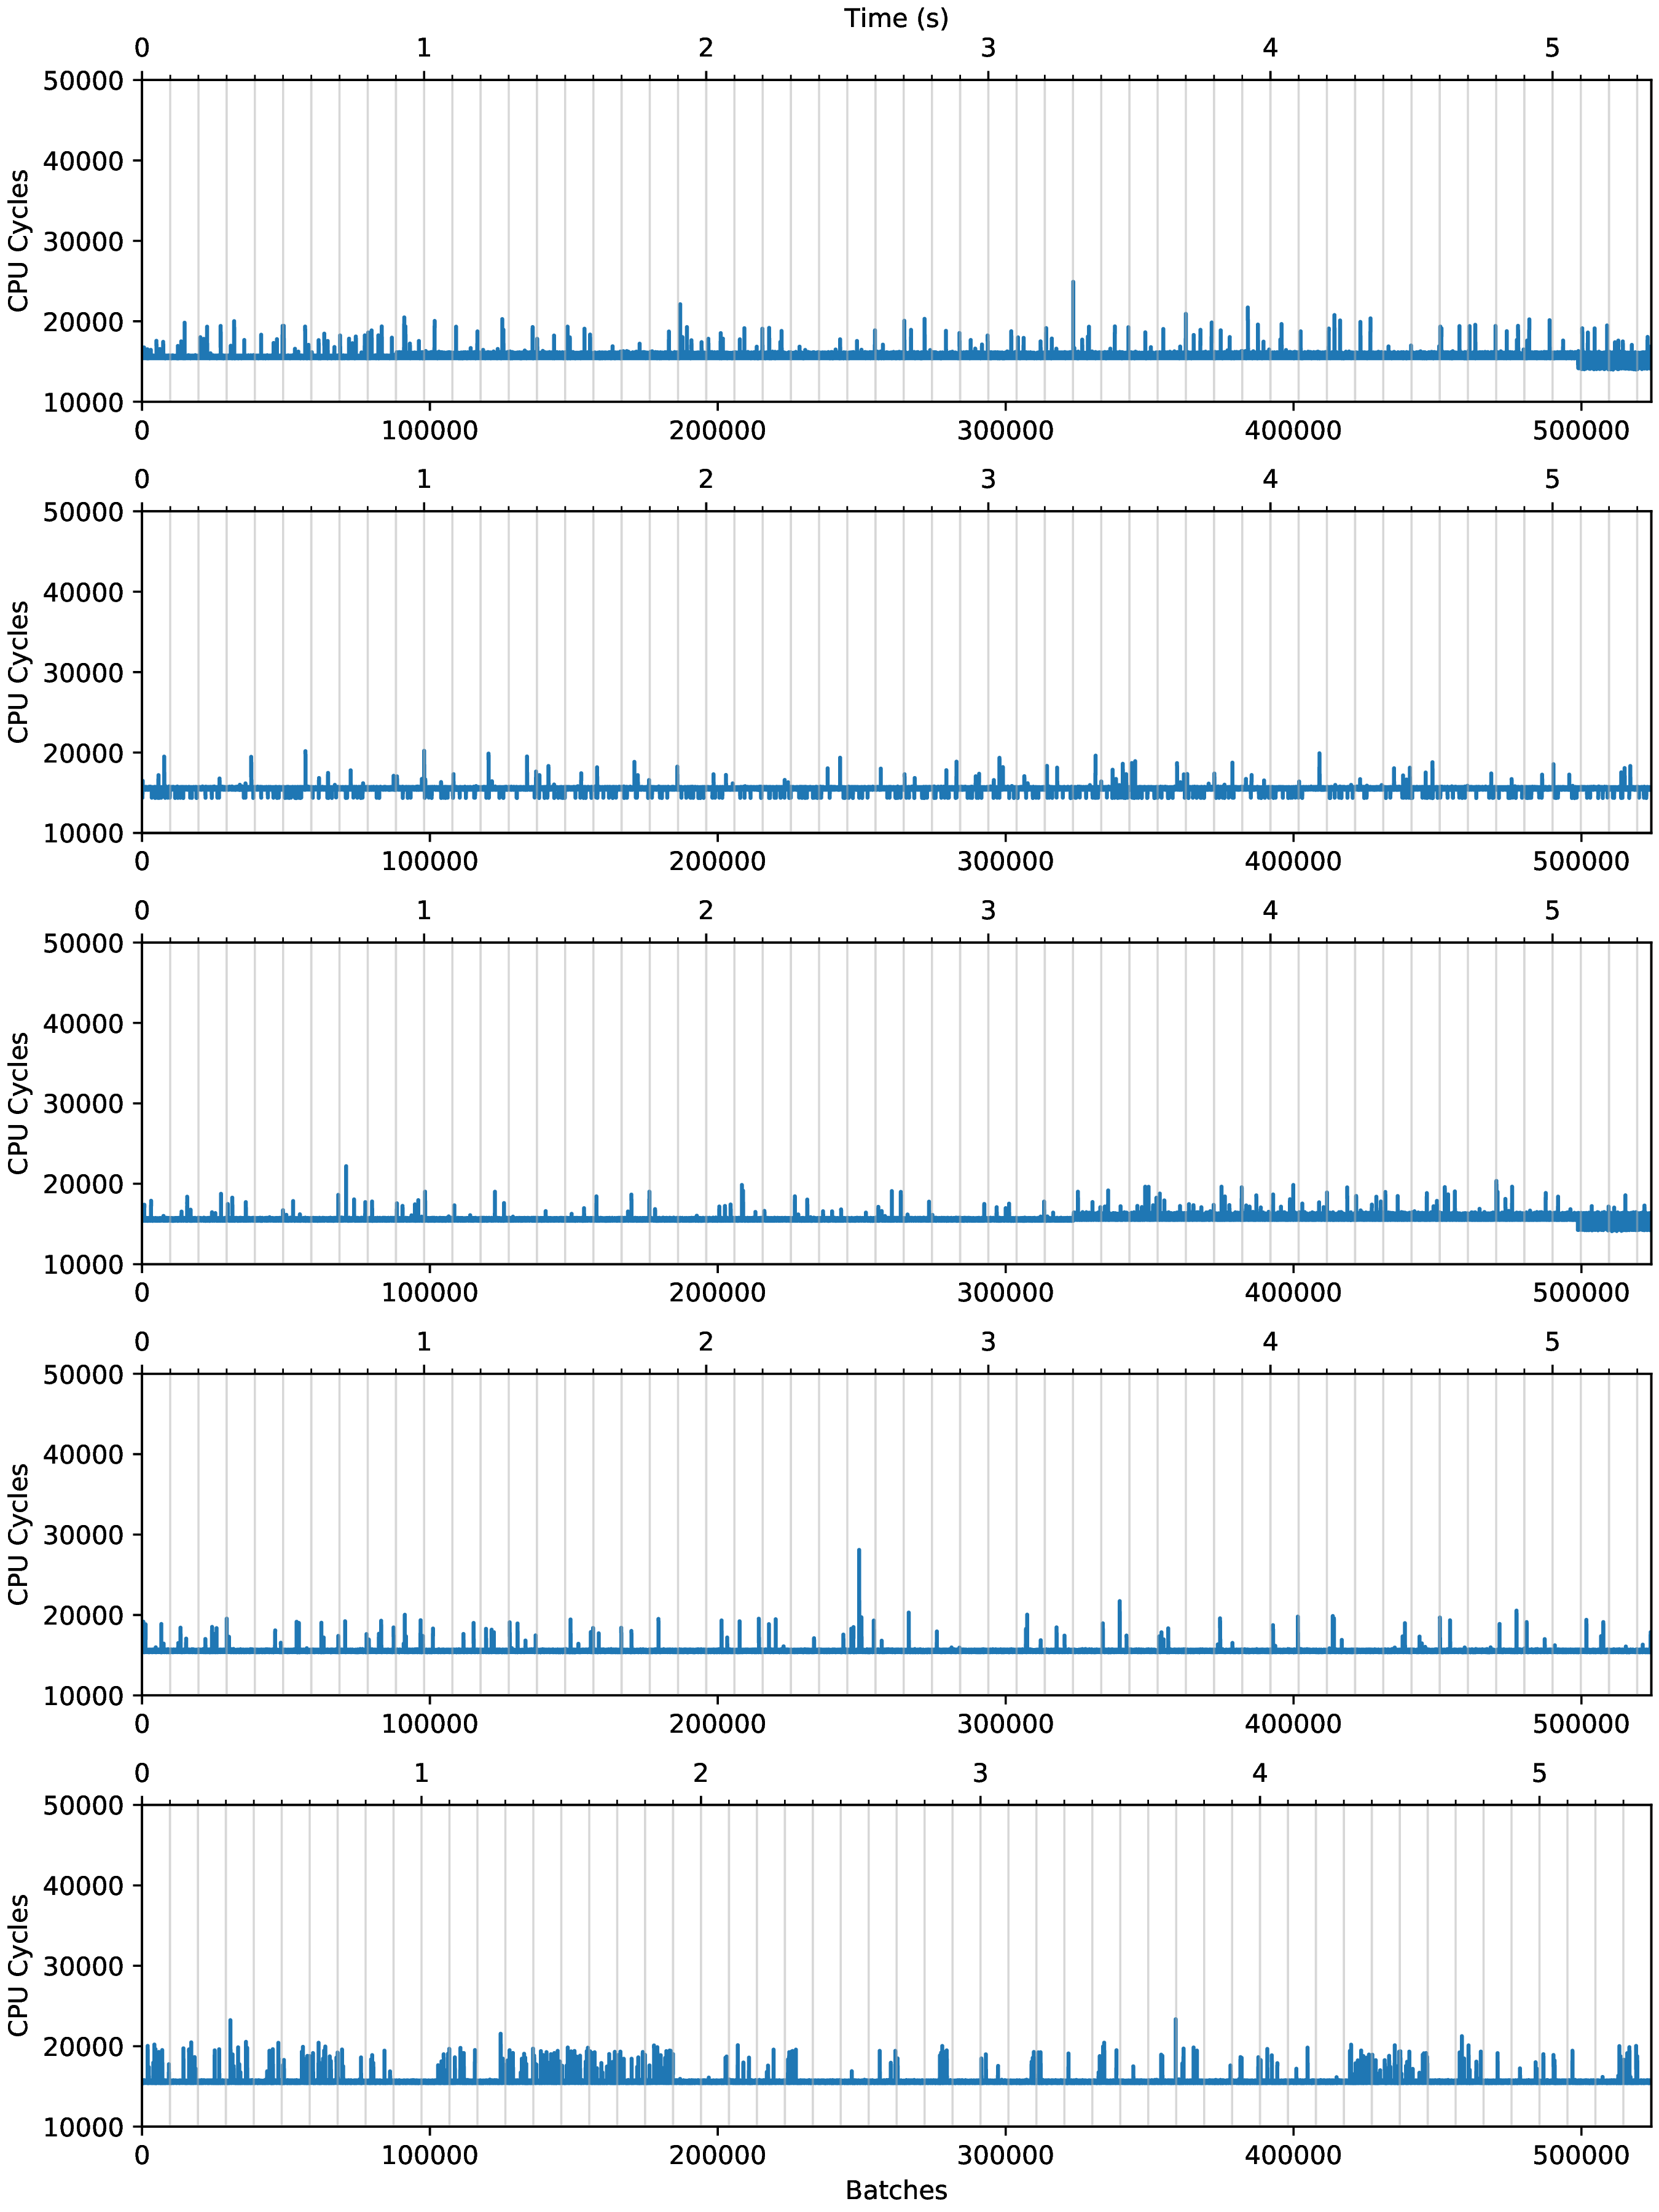
\includegraphics[width=0.7\textwidth,trim={0 52cm 0 0},clip]{figures/iotlb-baseline-iommu-pt-fixed-no-devs.png}
            \caption{CPU cycles per batch of transmitted packets with IOMMU and fixed
            virtual and physical addresses, other PCIe devices unbound.}
            \caption{}
        \end{figure}
    }

    \only<5>{
        \begin{figure}
            \centering
            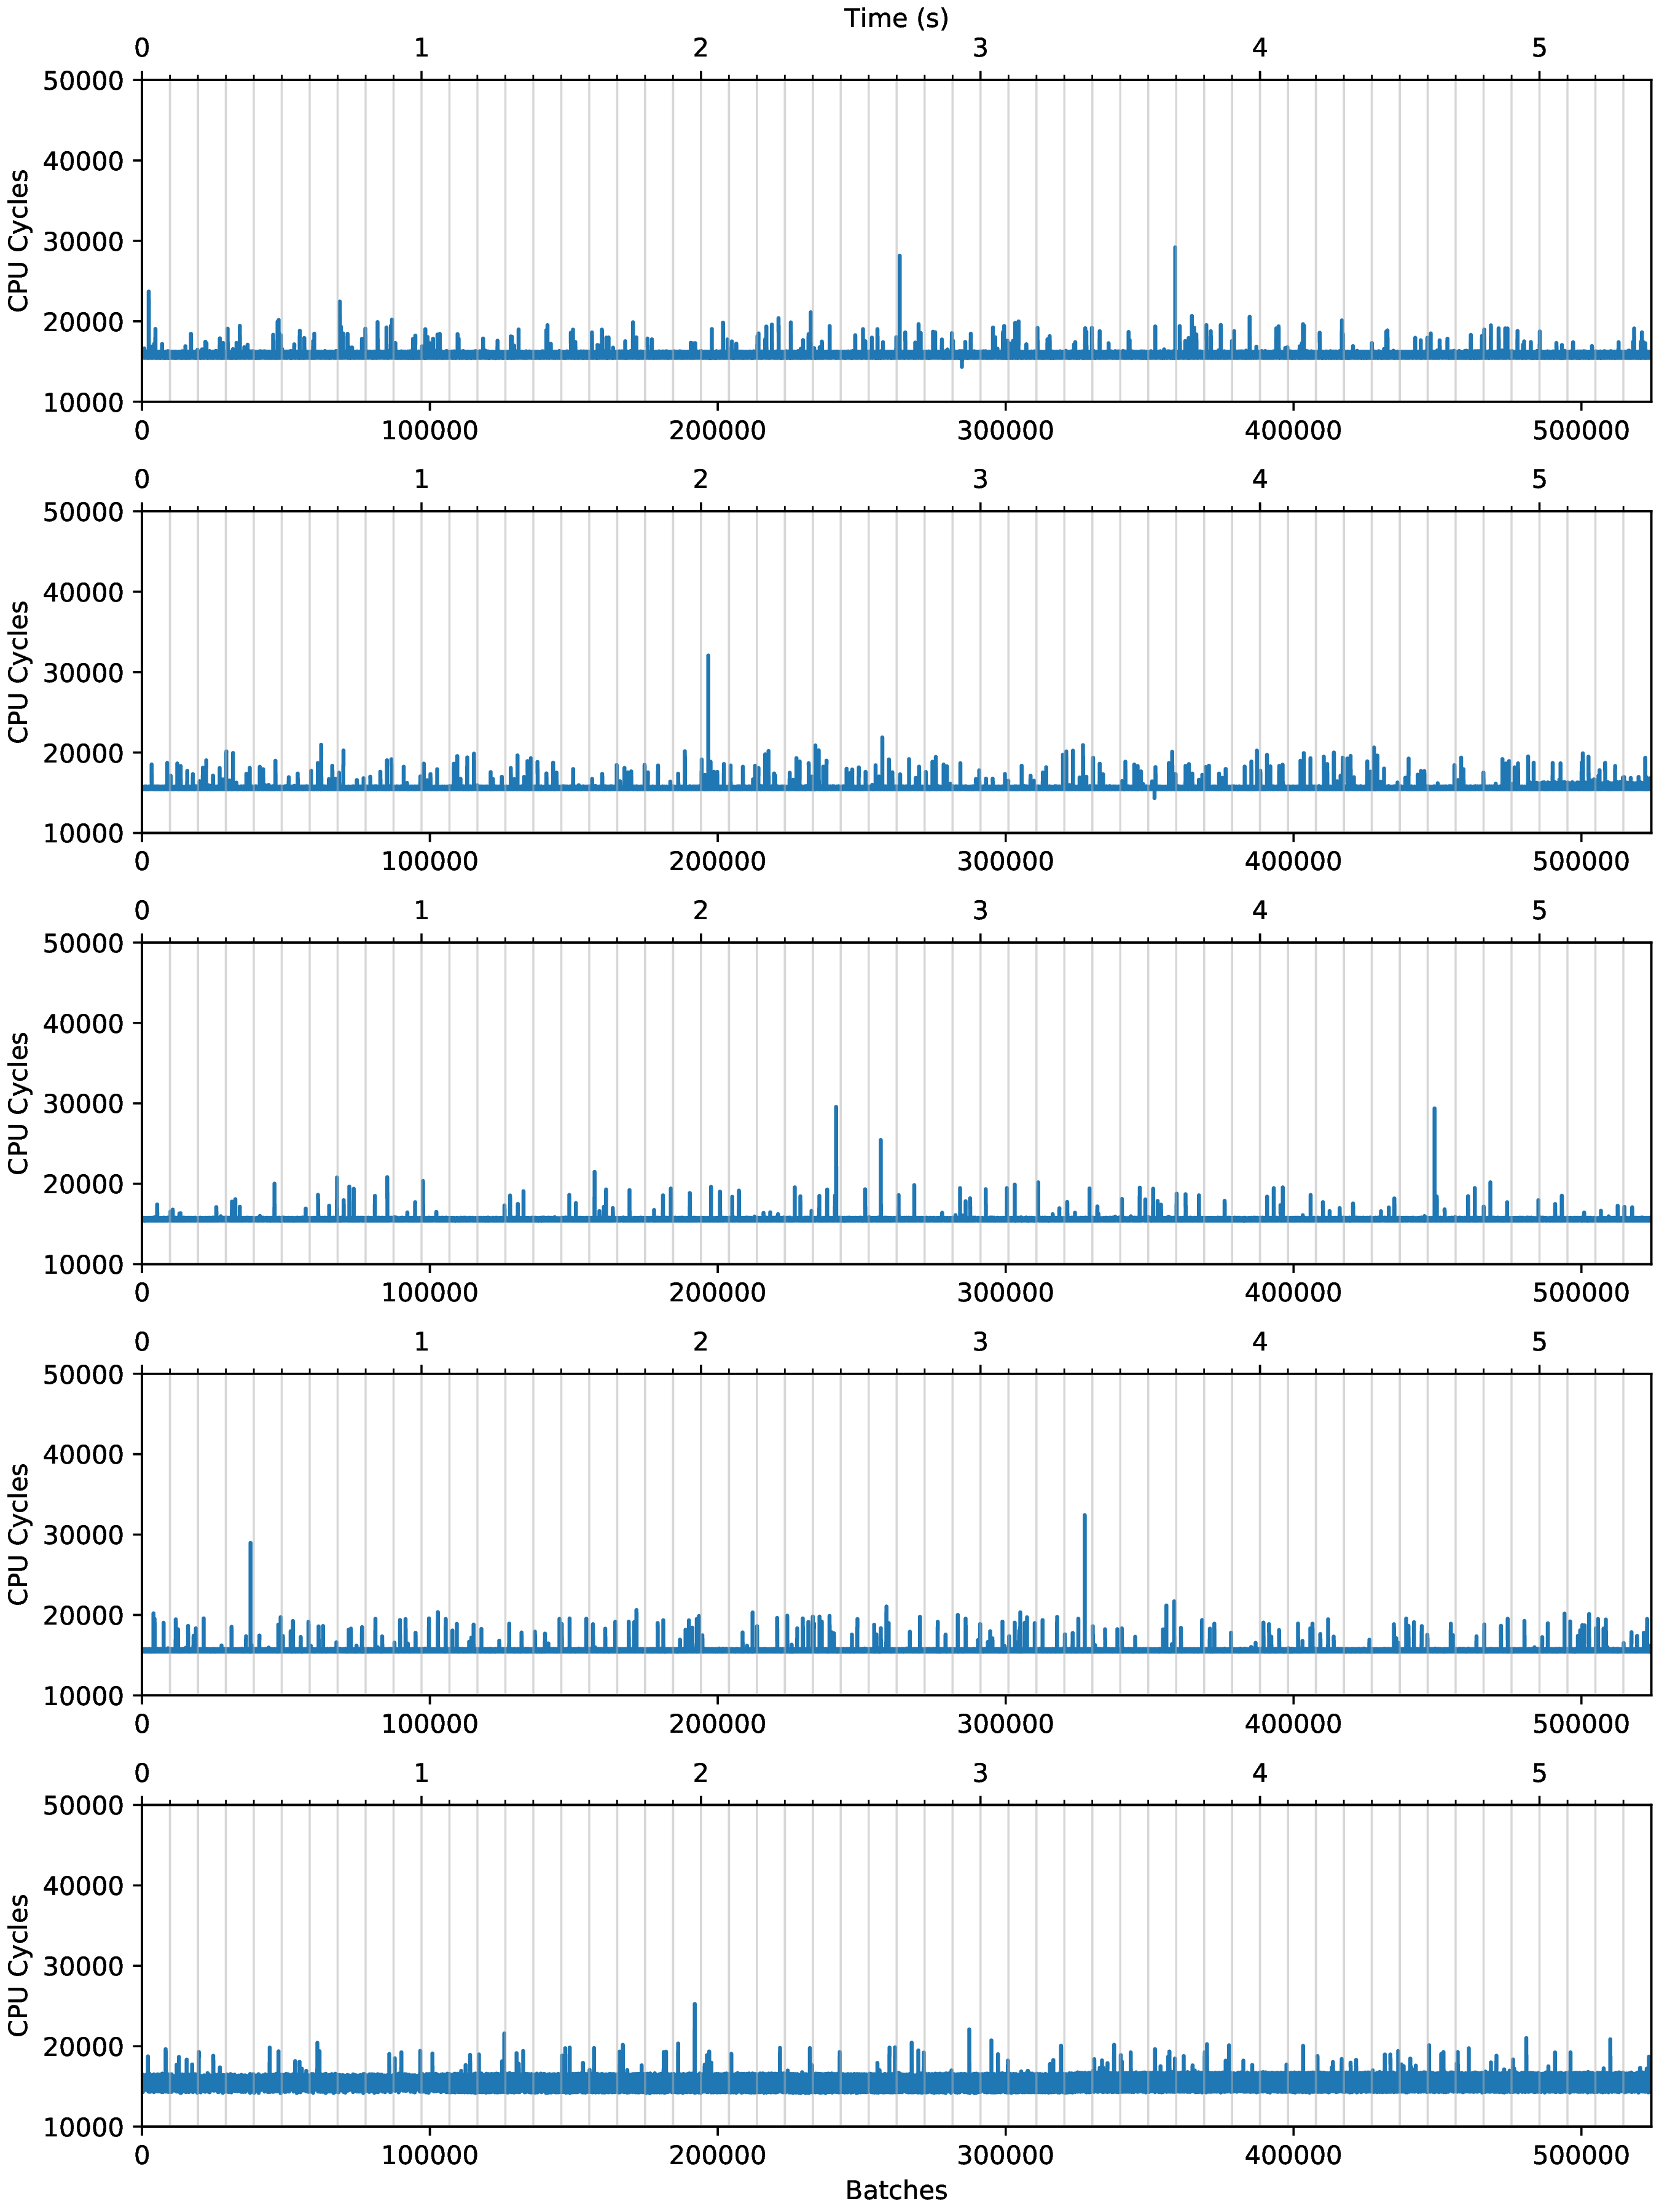
\includegraphics[width=0.7\textwidth,trim={0 52cm 0 0},clip]{figures/iotlb-baseline-iommu-pt-fixed-no-devs-ping-0.4.png}
            \caption{CPU cycles per batch of transmitted packets with IOMMU and
            fixed virtual and physical addresses, other PCIe devices unbound, ping
            on second NIC port every 0.4 seconds.}
        \end{figure}
    }

    \only<6>{
        Results:

        \begin{itemize}
            \item Measurements contain too much noise to detect any IOTLB misses
            \item Source for strongly varying number of CPU cycles for packet
                transmission is unclear
            \item Ideas on this topic very welcome
        \end{itemize}
    }
\end{frame}

\section{Conclusion}

\begin{frame}
    \begin{itemize}
        \item In most cases IOMMUs do not have a significant effect on throughput
            and latency
        \item However, in some cases throughput is strongly affected (decreases
            of more than 50\%!)
        \item Profileration of IOMMUs and support by OSes has increased sharply
        \item However, IOMMU protection against malicious internal hardware is
            still weak
    \end{itemize}
\end{frame}

\section{Contributions}

\begin{frame}
    ixy.rs:

    \begin{itemize}
        \item Driver for virtual functions (ixgbevf) to support SR-IOV
        \item Support for legacy Intel IOMMUs with IOVAs smaller than the host's
            virtual address widths
        \item Support for multiple devices associated to the same IOMMU group
        \item Bruteforce allocator to allocate physically and virtually
            contiguous memory on \SI{4}{\kibi\byte} pages
        \item A tool to perform timing measurements on the NIC's DMA operations
    \end{itemize}

    \vspace{1em}

    DPDK:

    \begin{itemize}
        \item Fixed an off-by-one-error in the ixgbe initialization code
    \end{itemize}
\end{frame}

